%%%%%%%%%%%%%%%%%%%%%%%%%%%%%%%%%%%%%%%%%%%%%%%%%%%%%%%%%%%%%%%%%%%%%%%%%%%%%%%
%% LaTeX-Vorlage für Abschlussarbeiten                                       %%
%% (TH Köln -Campus Gummersbach, Fak. 10)                                    %%
%%                                                                           %%
%% Gemäß dem Merkblatt zur Anfertigung von Projekt-, Bachelor-, Master- und  %%
%% Diplomarbeiten der Fakultät 10 von Frau Prof. Dr. Halfmann &              %%
%% Herr Prof. Dr. Rühmann (Version vom 27.01.2008)                           %%
%%                                                                           %%                                                                            
%% Bitte sprechen Sie unbedingt mit Ihrer Betreuerin bzw. Ihrem Betreuer     %%
%% bezüglich der Ausgestaltung Ihrer Arbeit!                                 %%
%%                                                                           %%
%%                                                                           %%
%% MERKKASTEN IN DIESER VORLAGE:                                             %%
%% In dieser Vorlage finden Sie Merkkasten, die Ihnen Informationen          %%
%% zu bestimmten, formalen Aspekten geben. Sprechen Sie immer auch mit       %% 
%% Ihrer Betreuerin bzw. Ihrem Betreuer dazu an.                             %%                       
%% Für die eigene Verwendung der Vorlage entfernen oder kommentieren Sie die %%
%% Merkkasten. Die betreffenden Bereiche für die Merkkasten in der Vorlage   %%
%% sind wie folgt kommentiert: <MERKKASTEN> ... </MERKKASTEN>.               %%                            %%                                                                           %%
%%                                                                           %%
%% LIZENZ:                                                                   %%
%% Diese Vorlage darf nicht kommerziell verbreitet                           %%
%% werden. Eine nicht-kommerzielle Weitergabe ist                            %% 
%% gestattet.                                                                %%
%%                                                                           %%
%% Von Ludger Schönfeld, M. Sc.,
%% 2014-2017                            %%
%%%%%%%%%%%%%%%%%%%%%%%%%%%%%%%%%%%%%%%%%%%%%%%%%%%%%%%%%%%%%%%%%%%%%%%%%%%%%%%

%%%%%%%%%%%%%%%%%%%%%%%%%%%%%%%%%%%%%%%%%%%%%
%% HEADER                                  %%
%%%%%%%%%%%%%%%%%%%%%%%%%%%%%%%%%%%%%%%%%%%%%
\documentclass[a4paper,12pt,oneside]{article}
% Optionen:
% - a4paper => DIN A4-Format
% - 12pt    => Schriftgröße (weitere  
%              grundlegende Fontgrößen: 10pt, 11pt)
% - oneside => Einseitiger Druck

%% Verwendete Pakete:
\usepackage[ngerman]{babel} % für die deutsche Sprache
\usepackage{caption} % Für schönere Bildunterschriften
\usepackage[T1]{fontenc} % Schriftkodierung (Für Sonderzeichen u.a.)
\usepackage[utf8]{inputenc} % Für die direkte Eingabe von Umlauten im Editor u.a.
\usepackage{fancyhdr} % Für Kopf- und Fußzeilen
\usepackage{lscape} % Für Querformat

%% Schriften (Beispiele)
%% Weitere LaTeX-Schriften im "LaTeX Font Catalogue"
%% unter: http://www.tug.dk/FontCatalogue/.
%% ACHTUNG: Ggf. müssen Schriften noch installiert 
%% werden!

% Serifen-Schriften:
\usepackage{lmodern} % Schriftart "Latin Modern"
%\usepackage{garamond} % Schriftart "Garamond"

%Sans Serif-Schriften:
%\usepackage[scaled]{uarial}
%\usepackage[scaled]{helvet}
%%--------------
\usepackage[normalem]{ulem} % Für das Unterstreichen von Text z.B. mit \uline{}
\usepackage[left=3cm,right=2cm,top=1.5cm,bottom=1cm,
textheight=245mm,textwidth=160mm,includeheadfoot,headsep=1cm,
footskip=1cm,headheight=14.599pt]{geometry} % Einrichtung der Seite 

\usepackage{graphicx} % Zum Laden von Graphiken
\usepackage{subcaption}
% INFO: Graphiken einbinden
%
% \includegraphics[scale=1.00]{dateiname}
%
% => Ausgabeformat: PDF-Dokument:
%    Es können die folgenden (Graphik-)formate eingebunden
%    werden: .jpg, .png, .pdf, .mps
% 
% => Ausgabeformat: DVI/PS:
%    Folgende (Graphik-)formate werden unterstützt:
%    .eps, .ps, .bmp, .pict, .pntg
\usepackage{epstopdf}

% Pakete für Tabellen
\usepackage{tabularx} % Einfache Tabellen
\usepackage{longtable} % Tabellen als Gleitobjekte (für die Aufteilung bei langen 
 %Tabellen über mehrere Seiten)
\usepackage{multirow} % Für das Verbinden von Zeilen innerhalb einer Tabelle mit
 % \multirow{anzahl}{*}{Text}

% (Zusatz-)Pakete für Formeln
\usepackage{amsmath}
\usepackage{amsthm}
\usepackage{amsfonts}

\usepackage{setspace} % Paket zum Setzen des Zeilenabstandes
% INFO: Zeilenabstand setzen:
%
% Befehle:
% - \singlespacing  => 1-zeilig (Standard)
% - \onehalfspacing => 1,5-zeilig
% - \doublespacing  => 2-zeilig 
\onehalfspacing % Zeilenabstand auf 1,5-zeilig setzen

% Farbboxen (für die Merkkästen in dieser Vorlage):
\usepackage{tcolorbox}
\tcbset{colback=white,colframe=orange,
        fonttitle=\bfseries}

\usepackage[colorlinks,pdfpagelabels,pdfstartview=FitH,
bookmarksopen=true,bookmarksnumbered=true,linkcolor=black,
plainpages=false,hypertexnames=false,citecolor=black]{hyperref} % Für Verlinkungen
% INFO: Verlinkungen mit dem hyperref-Paket:
%
% Die Angabe von URLs mit dem Befehl \url{} erlaubt einen
% gesonderten Umgang mit Weblinks. Denn die Links werden verlinkt.
% Auch erfolgt automatisch am Zeilenende ein Umbruch des Links.
% Es ist auch nicht erforderlich, Sonderzeichen in der URL manuell zu 
% entschärfen.
%
% TIPP: Sollte ein Umbuch bei einem Link nicht automatisch erfolgen, so kann
% das daran liegen, dass ein/mehrere Zeichen zusätzlich angegeben werden müssen,
% an dem der Link umbrochen werden kann.
% Dies kann mit folgendem Befehl erfolgen (Beispiel):
% \renewcommand*\UrlBreaks{\do-\do_}

% Das Paket "biblatex" für autom. 
% Literaturverzeichnisse:
%\usepackage{csquotes} % Für sprachangepasste Anführungszeichen
%\usepackage[backend=bibtex,style=alphabetic]  
%           {biblatex}
%\addbibresource{bib/literatur.bib}      

\usepackage{titlesec}
\usepackage{tocloft}

%\setcounter{tocdepth}{5} % Set the depth for table of contents
%\setcounter{secnumdepth}{5} % Set the depth for numbered sections

\titleformat{\paragraph}
{\normalfont\normalsize\bfseries}{\theparagraph}{1em}{}
\titlespacing*{\paragraph}
{0pt}{3.25ex plus 1ex minus .2ex}{1.5ex plus .2ex}

\titleformat{\subparagraph}
{\normalfont\normalsize\bfseries}{\thesubparagraph}{1em}{}
\titlespacing*{\subparagraph}
{0pt}{3.25ex plus 1ex minus .2ex}{1.5ex plus .2ex}[0pt]

\renewcommand{\cftparaindent}{70pt} % Decrease indentation for \paragraph in table of contents
\renewcommand{\cftsubparaindent}{90pt} % Decrease indentation for \subparagraph in table of contents

% für Anführungszeichen z.B. \enquote{abc}
\usepackage{csquotes}

\usepackage{float} % for the 'H' specifier

\usepackage{pgfplots} % for plots

%%%%%%%%%%%%%%%%%%%%%%%%%%%%%%%%%%%%%%%%%%%%%
%% DOKUMENT                                %%
%%%%%%%%%%%%%%%%%%%%%%%%%%%%%%%%%%%%%%%%%%%%%
\begin{document}
  % Unbeschriftetes Vorblatt (Leere Seite)
  \pagestyle{empty} % Seite ohne Kopf- und Fußzeilen
  \newpage % Neue Seite
  %\newpage
\thispagestyle{empty}
\section*{}
  % Ausgelagerte LaTeX-Datei (hier: leereSeite.tex) einbinden
  
  % Deckblatt
  \pagestyle{empty}
  \begin{titlepage}
    
\includegraphics[scale=1.00]{Sources/logo_TH-Koeln_CMYK_22pt}\\
    \begin{center}
      \Large
      Technische Hochschule Köln\\
      Fakultät für Informatik und Ingenieurwissenschaften\\
      \hrule\par\rule{0pt}{2cm} % Horizontale Trennlinie  mit 2 cm Abtand nach unten erzeugen
      \LARGE
      \textsc{P R A K T I K U M}\\
      \vspace{1cm} % Vertikaler Abstand von 1cm erzeugen
      \huge
      Neuronale Netze\\
      \Large
      Gruppe M.16\\
      \vspace{1.5cm}
      \large
      Vorgelegt an der TH Köln\\
      Campus Gummersbach\\
      %im Modul\\
      Mathematik 2\\ 
      \vspace{1.0cm}
      ausgearbeitet von:\\
      \begin{tabular}{c}
        \textsc{Maximilian Luca Ramacher}
      \end{tabular}
      \begin{tabular}{c c}
        \textsc{Marius Kühnast} &
        \textsc{Muratcan Garanli}\\
        \textsc{Kai Murza} &
        \textsc{Nick Struckmeyer}\\
      \end{tabular}\\
      \vspace{1.5cm}
      \begin{tabular}{ll} % Einfache Tabelle ohne Rahmen, mit 2 Spalten erzeugen
          \textbf{Erster Betreuer:} & Marc Oedingen \\
          \textbf{Zweiter Betreuer:} & Peter Wagner \\
      \end{tabular}
      \vspace{1.5cm}
      \\Gummersbach, im Juni 2023
    \end{center}    
  \end{titlepage}

  %Abstract
  %\newpage
  % Abstract (ACHTUNG: Abweichung zur Reihenfolge im Merkblatt!)
  %\begin{abstract}
  %  Platz für das deutsche Abstract...
  %\end{abstract}
  
  %\renewcommand{\abstractname}{Abstract}
  %\begin{abstract}
  %  Platz für das englische Abstract...
  %\end{abstract}


  % %<MERKKASTEN> (für die eigene Verwendung bitte entfernen
  %   \vspace{1cm}
  % \begin{tcolorbox}[title={Das Abstract}]
  % Bei einem Abstract handelt es sich um eine Art \textit{Zusammenfassung} Ihrer Arbeit. Diese kann in deutscher und/oder englischer Sprache verfasst werden. Mithilfe des Abstracts kann der Leser sich zügig orientieren, in wie fern Ihre Arbeit für ihn Relevanz besitzt.\\                                                                      Sprechen Sie unbedingt mit Ihrer Betreuerin/Ihrem Betreuer, ob Sie für Ihre Arbeit ein Abstract benötigen.\\
  % Ein Abstract beinhaltet folgende Aspekte \footnote{ Vgl. \cite{SW11}, S. 249}:
  % \begin{itemize}
  %   \item Ziel der Arbeit
  %   \item Fragestellung der Arbeit
  %   \item Herangezogener, theoretischer Ansatz ("Quellen")
  %   \item \textit{Optional:} Methodik
  % \end{itemize}
  % \end{tcolorbox}
  % %</MERKKASTEN>

  % %<MERKKASTEN> (für die eigene Verwendung bitte entfernen
  %  \vspace{1cm}
  %   \begin{tcolorbox}[title={Hinweise zu dieser Dokumentvorlage}]
  %   \begin{itemize}
  %   \item Es handelt sich hierbei um eine Beispiel-Vorlage für wissenschaftliche Ausarbeitungen.
  %     Über die konkrete, formale Ausgestaltung Ihrer wissenschaftlichen Arbeit sprechen Sie unbedingt mit Ihre/m Betreuer/in.
  %   \item Unabhängig, ob Sie beispielsweise eine Bachelor-, Master- oder Hausarbeit schreiben müssen. Diese Vorlage kann als eine gute Basis für Ihre Arbeit dienen. Passen Sie einfach die Vorlage Ihren Anforderungen entsprechend an.
  %   \end{itemize}
  %   \end{tcolorbox}
  %   %</MERKKASTEN>  
  
  % Inhaltsverzeichnis
  \newpage
  \tableofcontents
  
  \newpage
  \pagestyle{fancy} % Kopf- und Fußzeilen aktivieren (=> Paket "fancyhdr")
  
  % Abbildungsverzeichnis  
  % INFO: Abbildung einbinden (Beispiel):
  %  \begin{figure}[h!]
  %    \centering
  %    \includegraphics[scale=1.00]{Pfad zum Bild}\\
  %    \caption{Bildunterschrift} 
  %    \label{Marke zum Referenzieren auf die Abbildung}
  %  \end{figure}

  \section*{Abbildungsverzeichnis}
  \addcontentsline{toc}{section}{Abbildungsverzeichnis} % Manuellen Eintrag im Inhaltsverzeichnis erzeugen
  \renewcommand{\listfigurename}{} % Name des Abbildungsverzeichnisses ändern
  \thispagestyle{empty}
  \listoffigures
  
  %\newpage
  % Tabellenverzeichnis
  %\addcontentsline{toc}{section}{Tabellenverzeichnis}
  %\listoftables
  
  %\newpage

  % Hauptteil des Dokuments
  % TIPP: Jedes Kapitel oder jeder Abschnitt in eine eigene
  % LaTeX-Datei (.tex) auslagern.
  % Einbinden der ausgelagerten Dateien in diese Hauptdatei, erfolgt 
  % mittels folgendem Befehl (Beispiel):
  % beispiel.tex => \input{beispiel}
  % INFO: Querverweise auf Gliederungselemente, Abbildungen 
  %       & Tabellen setzen:
  %
  % Voraussetzung: Gesetzte Referenzmarke mit dem Befehl: \label{marke}
  % 
  % Referenzierung erfolgt dann mittels dem Befehl:
  % \ref{marke}
  \newpage
\thispagestyle{empty}
\section{Einleitung Neuronale Netze}\label{sec:einleitung_nn}   

\vspace{1cm}

\begin{tcolorbox}[title={Inhalt}]
  \begin{quotation}\noindent
      Dieses Kapitel liefert einen Einstieg in neuronale Netze. Es werden an Beispielen unterschiedliche Anwendungsfälle anschaulich gemacht.
      Ebenso soll bereits eine grobe Idee näher gebracht werden, wie ein neuronales Netz aufgebaut ist.
      Insgesamt werden in diesem Kapitel bereits zahlreiche grundlegende Begriffe erklärt, die in den nachfolgenden Kapiteln benötigt werden.
  \end{quotation}
  \begin{itemize}  
    \item Wofür benötigt man Neuronale Netze?
    \item Einsatzgebiete
    \item Grobes Prinzip
  \end{itemize}
\end{tcolorbox}

\subsection{Wofür benötigt man Neuronale Netze?}\label{subsec:einleitung_nn:wofuer_nn}
Mit neuronalen Netzen lassen sich Probleme lösen, die mit herkömmlichen Algorithmen nur schwer bis gar nicht lösbar sind. Neuronale Netze sind grundsätzlich in der Lage, nichtlineare Abbildungen anzunähern, Beispiele folgen weiter unten (siehe \ref*{subsec:einleitung_nn:einsatzgebiete}).
Der große Vorteil neuronaler Netze liegt darin, dass sie selbstständig lernen können, Muster in Daten zu erkennen, wodurch man die entsprechenden Algorithmen nicht mehr von Hand schreiben muss.
Neuronale Netze sind dabei in der Lage, auch komplexe Muster und Zusammenhänge aus sehr großen Datenmengen zu erkennen und zu extrahieren.

\bigbreak\noindent
Aufgrund ihrer Fähigkeit, schnell und effizient komplexe Muster zu erkennen, können neuronale Netze auch Aufgaben lösen, für die man normalerweise Menschen benötigen würde, da herkömmliche Algorithmen diese Probleme nicht zuverlässig genug lösen können oder der Entwicklungsaufwand unverhältnismäßig groß in Relation zum Nutzen wäre.

\bigbreak\noindent
Häufig sind Muster zu komplex, um sie mit einem klassischen Algorithmus erfassen zu können oder sie sind schlecht von Hand mathematisch formulierbar.
Ein Beispiel hierfür wäre die Erkennung von Tieren auf einem Foto. Die Eigenschaften, die z.B. eine Katze ausmachen von Hand in Bedingungen zu überführen ist nahezu unmöglich, gerade deswegen da die Katzen sehr verschieden aussehen können und aus verschiedenen Perspektiven auf dem Foto zu sehen sein können und die Menge an Merkmalen viel zu groß und komplex ist.
Mit Hilfe eines neuronalen Netzes kann man aber dennoch mit relativ geringem Aufwand ein Netz trainieren, das in der Lage ist, solche Bilderkennungsaufgaben zu erledigen.

\bigbreak\noindent
Neuronale Netze sind häufig auch zuverlässiger bei der Lösung eines Problems, als klassische Algorithmen, da herkömmliche Algorithmen manchmal bestimmte Sonderfälle nicht abdecken können, wohingegen neuronale Netze anpassungsfähiger sind und teilweise mit solchen Sonderfällen umgehen können, da sie diese Fälle aus ihren Trainingsdaten extrahieren konnten, ein menschlicher Entwickler diese aber bei der Entwicklung eines Algorithmus übersehen hätte.
Ein Beispiel für solche Fälle könnten autonom fahrende Fahrzeuge sein.
Bei diesen ist es schwer möglich, Algorithmen zu schreiben, die unter allen Wetter-, Straßen- und Umweltbedingungen zuverlässig funktionieren.
Schlecht zu sehende Straßenschilder oder Straßen mit undeutlichen Markierungen könnten ein Problem für solche Algorithmen darstellen, da handgeschriebene Algorithmen meistens auf genau solche Straßenmerkmale angewiesen sind.
Neuronale Netze hingegen können möglicherweise mit solchen Fällen umgehen könnten, da sie sich aus den Trainingsdaten mehrere Faktoren abgeleitet haben, an denen sie sich orientieren können und zuverlässiger in der Erkennung von Mustern wie Straßenschildern sind.

\subsection{Einsatzgebiete}\label{subsec:einleitung_nn:einsatzgebiete}
Neuronale Netze sind äußerst vielfältig und lassen sich für verschiedenste Anwendungen anpassen und trainieren.
Zu den häufigsten Anwendungsfällen zählen die Bilderkennung und die Verarbeitung von auditiven Daten.

\bigbreak\noindent
Die Bilderkennung mittels neuronaler Netze lässt sich beispielsweise dazu einsetzen, medizinische Diagnosen durchzuführen, da diese Netze fähig sind, komplexe Krankheitsbilder zu erkennen.
Röntgenbilder können von neuronalen Netzen auf Anzeichen von Tumoren untersucht werden und können so medizinisches Fachpersonal bei Ihrer Arbeit unterstützen.
Auch kann die Bilderkennung genutzt werden, um die Position von Personen oder anderen Objekten auf einem Kamerabild zu identifizieren, was zur Realisierung von autonomem Fahren nützlich ist.
Dabei werden vor allem sogenannte “convolutional neural networks” verwendet.
Dabei handelt es sich um eine Variante von neuronalen Netzen, die auf Grund der speziellen verwendeten Schichten und Aktivierungsfunktionen besonders gut für die Bilderkennung geeignet sind.
Die Bilderkennung mittels neuronaler Netze findet auch in der Industrie Anwendung, um hergestellte Produkte automatisiert auf Mängel zu prüfen und auszusortieren.

\bigbreak\noindent
Neuronale Netze können auch eingesetzt werden, um das Verhalten von Menschen zu analysieren. Anhand von Analytik Daten über die Interaktionen von Nutzern mit beispielsweise einer Website lassen sich mittels neuronaler Netze an den Nutzer angepasste Empfehlungen für Produkte, Videos oder ähnliches generieren.
Die großen Mengen von anfallenden Daten über Nutzerinteraktionen können von solchen Netzen gefiltert und verarbeitet werden, um Muster im Verhalten der Nutzer zu finden, wodurch man auf die Vorlieben des Anwenders Rückschlüsse ziehen kann.

\bigbreak\noindent
Neuronale Netze sind grundsätzlich in der Lage, beliebige Arten von Eingabedaten zu verarbeiten.
So ist es auch möglich, Audio-Daten zu verarbeiten und so beispielsweise Spracherkennung, automatisch generierte Untertitel und Sprachassistenten zu implementieren.

\subsection{Grobes Prinzip}\label{subsec:einleitung_nn_grobes:prinzip}
Neuronale Netze orientieren sich an der Funktionsweise von menschlichen Gehirnen und versuchen dadurch eine ähnliche Lernfähigkeit zu erzielen.
Dabei werden Netze aus Neuronen simuliert, um menschliche Lernprozesse und kognitive Fähigkeiten nachzuahmen. 

\bigbreak\noindent
Die Neuronen neuronaler Netze sind in Schichten organisiert, die untereinander verbunden sind.
Bei einem sogenannten ''feed-forward'' neuronalen Netz werden die Signale dabei von den Ausgängen der Neuronen der einen Schicht zu den Eingängen der Neuronen der nächsten Schicht geleitet.

\bigbreak\noindent
Neuronen implementieren Funktionen, die die Eingabedaten verarbeiten und ein Ausgabesignal liefern, die sogenannten Aktivierungsfunktionen.
Dabei werden zunächst die Eingabedaten zusammengefasst, meist indem sie aufsummiert werden und anschließend wird eine Aktivierungsfunktion auf das Ergebnis angewendet. Dadurch soll eine nicht-linearität mit eingebracht und die Werte auf einen bestimmten Wertebereich beschränkt werden.

\bigbreak\noindent
Die Verbindungen zwischen den Neuronen sind von variabler Stärke und sind der primäre Faktor, der beim Lernprozess verändert wird.

\bigbreak\noindent
Neuronale Netze werden trainiert, indem man sie auf einen Trainingsdatensatz anwendet und die Verknüpfungen der Neuronen anpasst.
Der Trainingsdatensatz enthält dabei beispielhafte Eingabedaten und die dazugehörige gewünschte Ausgabe.

\bigbreak\noindent
Basierend auf der Abweichung der Ergebnisse des neuronalen Netzes von denen der Trainingsdaten werden die Verknüpfungen der Neuronen dann automatisiert angepasst, wodurch ein Lerneffekt erzielt wird.
Dazu wird das Gradientenverfahren eingesetzt, damit die Optimierung des Netzes möglichst schnell geschieht.
Nachdem das Netz trainiert wurde, kann man es dann mit Daten speisen, die noch nicht in den Trainingsdaten enthalten waren und das Netz bildet dann eine entsprechende Ausgabe, basierend auf den Zusammenhängen, die es aus dem Trainingsdatensatz extrahiert hat.


%Neuronen 
\newpage  
\section{Neuronen}\label{sec:neuronen}
  \begin{tcolorbox}[title={Inhalt}]
\begin{itemize} 
    \item Was sind Neuronen
    \item Arten von Neuronen
    \item Funktionsweise
    \item Aktivierungsfunktion
    \item Schichtenmodell
\end{itemize} 
\end{tcolorbox}
\subsection{Was sind Neuronen?}\label{sec:neuronen:was_sind_neuronen}  
Das menschliche Nervensystem besteht aus Neuronen, welche mit Axonen oder Dendriten verknüpft sind. Diese Verbindungen werden auch Synapsen genannt. Die variable Stärke der Synapsen
ermöglichen das Lernen. Dieser biologische Mechanismus wird durch neurale Netze simuliert.\\

\begin{figure}[H]
\begin{subfigure}{0.6\textwidth}
    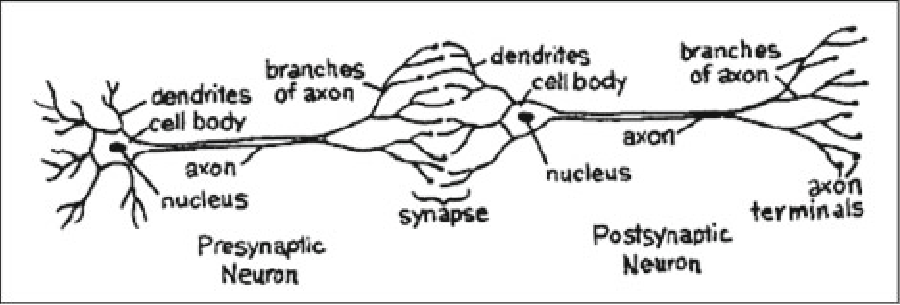
\includegraphics[width=\textwidth]{Sources/01-01_synapse.png}
    \label{Synapse}
    \caption{Synapse}
\end{subfigure}
\begin{subfigure}{0.25\textwidth}
    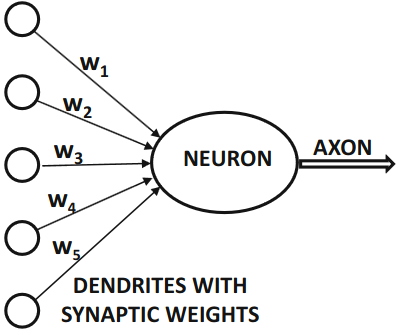
\includegraphics[width=\textwidth]{Sources/01-02_neuron.png}
    \label{Neuron}
    \caption{Neuron}
\end{subfigure}
\caption{Neural Networks and Deep Learning A Textbook, Charu C. Aggarwal
}
\end{figure}

Eines neuronales Netz besteht aus mindestens einem Neuron. Neuronen sind essentielle Bestandteile von neuralen Netzen. Sie nehmen Eingabedaten entgegen und wandeln diese 
in Ausgabedaten um. Neben den Eingabedaten werden auch Weight-Parameter übergeben, welche die zu berechnenden Werte beinflussen. Das eigenliche \enquote{Lernen} erfolgt durch diesen 
Einfluss.
\subsection{Arten von Neuronen}\label{subsec:neuronen:arten_von_neuronen}
  TEXT FOLGT... 
\newpage
\subsection{Funktionsweise}\label{subsec:neuronen:funktionsweise}
  
\subsubsection{Perceptrons}
Die simpelste Form eines Neuralen Netzwerks ist ein Perceptron. Es kann nur binäre Entscheidungen \{-1,+1\} treffen. Ein Perceptron besteht aus einer Input Layer und einem Output Node.
Die Input Layer beinhaltet $d$ nodes welches $d$ Merkmale $\overline{X} = [x_1...x_d]$ mit Weights $\overline{W} = [w_1...w_d]$ übermittelt. Die lineare Aktivierungsfunktion sign berechnet
dann die Vorhersage $\hat{y}$. \\
$$\hat{y} = sign\{\overline{W} \cdot \overline{X}\} = sign\{\sum\limits^{d}_{j=1}w_jx_j\}$$\\
In vielen Fällen wird ein nicht variables Element $b$ mit in der Rechnung berücksichtigt. Dies verursacht das der Mittelwert der Vorhersage nicht 0 ist.\\
$$\hat{y} = sign\{\overline{W} \cdot \overline{X} + b\} = sign\{\sum\limits^{d}_{j=1}w_jx_j + b\}$$\\
\begin{figure}[H]
    \begin{subfigure}{0.5\textwidth}
        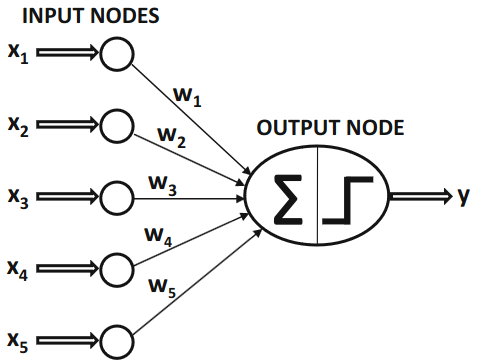
\includegraphics[width=\textwidth]{Sources/02-01_perceptron.png}
        \label{Synapse}
        \caption{{Perceptron ohne Bias}}
    \end{subfigure}
    \begin{subfigure}{0.5\textwidth}
        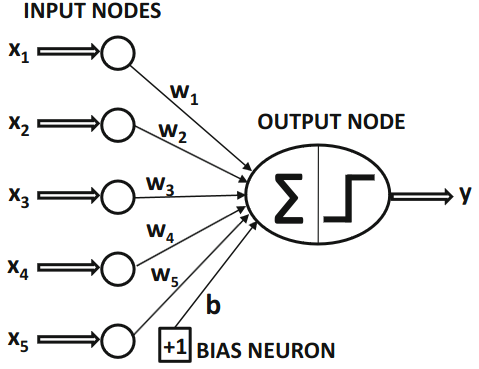
\includegraphics[width=\textwidth]{Sources/02-02_perceptronMitBias.png}
        \label{Neuron}
        \caption{Perceptron mit Bias}
    \end{subfigure}
    \caption{Aufbau von Perceptronen, Bild aus dem Buch 'Neural Networks and Deep Learning' von Charu C. Aggarwal
    }
    \end{figure}

\noindent 
Durch der so genannten Minimierung lässt sich der Fehler der Vorhersage verringern. Hierzu werden neben den Features x, auch Labels y in einem Feature-Label Paar eingeführt. 
$$\text{Minimize}_{\overline{W}}L = \sum\limits_{(\overline{X},y)\in \mathcal{D}}(y - \hat{y})^2 = \sum\limits_{(\overline{X},y)\in \mathcal{D}}(y - sign\{\overline{W} \cdot \overline{X}\})^2$$
Diese Art der Minimierung wird auch als Loss-Funktion bezeichnet. Die obige Funktion führt zu einer treppenstufigen Loss-Ebene, welche für gradient-descent ungeignet ist. Um diesem Problem entgegen zu wirken, wird eine Smooth-Funktion angewendet.
$$\Delta L_{\text{smooth}} = \sum\limits_{(\overline{X},y)\in \mathcal{D}}(y - \hat{y})\overline{X}$$
Beim Trainieren eines Neuralen Netzwerks werden Eingabedaten $\overline{X}$ einzelt oder in kleinen Batches eingespeist um die Vorhersage $\hat{y}$ zu generieren. Die Weights werden dann durch den Fehlerwert $E(\overline{X}) = (y - \hat{y})$ aktualisiert.
$$\overline{W} \Rightarrow \overline{W} + \alpha(y - \hat{y})\overline{X}$$
Der Parameter $\alpha$ reguliert die Lernrate des Neuralen Netzwerks. Der Perceptron-Algorithmus durchläuft die Trainingsdaten mehrmals bis die Weight-Werte konvergieren. Ein solcher Durchlauf wird als Epoche bezeichnet.\\
Der Perceptron-Algorithmus kann auch als stochastische Gradientenabstiegsmethode betrachtet werden. TODO Erklärung hier? 
 
\subsubsection{Aktivierungsfunktion}\label{subsec:neuronen:aktivierungsfunktion}
  Aktivierungsfunktionen ermöglichen den Neuronen nicht-lineare Outputs zu produzieren. Außerdem wird durch diese Funktionen entschieden, 
welche Neuronen aktiviert werden und wie die Inputs gewichtet werden. Zur Notation von Aktivierungsfunktion nutzen wir $\Phi$.
$$\hat{y} = \Phi(\overline{W} \cdot \overline{X})$$
\paragraph{Lineare Aktivierung}
Die simpelste Aktivierungsfunktion $\Phi(\cdot)$ ist die lineare Aktivierung. Sie bietet keine nicht linearität. Sie wird oft in Output Nodes
verwendet, wenn das Ziel ein reeler Wert ist.
$$\Phi(v) = v$$
\paragraph{Nicht lineare Aktivierung}
In den frühen Tagen der Entwicklung von neuralen Netzen wurden sign, sigmoid und hyperbolic tangent Funktionen genutzt.
\subparagraph{Sign Aktivierung}
Die sign Funktion generiert nur binäre \{-1,+1\} Ausgaben. Aufgrund der Nichtstätigkeit der Funktion, können beim Trainieren keine Loss-Funktionen verwendet werden.
$$\Phi(v) = \text{sign}(v)$$
\subparagraph{Sigmoid Aktivierung}
Die Sigmoid Funktion generiert Werte zwischen 0 und 1. Sie eignet sich deshalb für Rechnungen die als Wahrscheinlichkeiten interpetiert werden sollen.
$$\Phi(v) = \frac{1}{1 + e^{-v}}$$
\subparagraph{Tanh Aktivierung}
Der Graph der Tanh Funktion hat eine ähneliche Form wie die der Sigmoid Funktion. Sie unterscheidet sich jedoch in der Skalierung, denn ihre Wertebereich liegt zwischen -1 und 1.
$$\Phi(v) = \frac{e^{2v} - 1}{e^{2v} + 1}$$
Die Tanh Funktion lässt sich auch durch die Sigmoid Funktion darstellen.
$$\text{tanh}(v) = 2 \cdot \text{sigmoid}(2v) - 1$$
Wenn die Ausgabe der Berechnung postitiv sowie negativ sein kann, ist die tanh Funktion der sigmoid Funktion vorzuziehen. Außerdem ist es einfacher zu trainieren, weil die Funktion Mittelwertzentriert
und der Gradient größer ist.

\paragraph{Piecewise lineare Aktivierung}
Historisch wurden die Sigmoid und Tanh Funktion zur Einführung von Nichtliniearität genutzt. Heutzutage sind piecewise linear activation Funktionen (Stückweise Linear) beliebter, weil diese das Trainieren 
von mehrschichtigen neuronalen Netzen einfacher machen.
\subparagraph{ReLU}
TODO\\
$$\Phi(v) = \text{max}\{v,0\}$$
\subparagraph{hard tanh Aktivierung}
TODO\\
$$\Phi(v) = \text{max}\{\text{min}[v,1],-1\}$$

\begin{figure}[htbp]
    \centering
    \begin{subfigure}{0.3\textwidth}
      \centering
      \begin{tikzpicture}
        \begin{axis}[
          width=\textwidth,
          height=5cm,
          xmin=-2,
          xmax=2,
          ymin=-2,
          ymax=2
        ]
          \addplot[black, domain=-2:2, samples=100] {x};
        \end{axis}
      \end{tikzpicture}
      \caption{Linear}
      \label{fig:plot1}
    \end{subfigure}
    \hfill
    \begin{subfigure}{0.3\textwidth}
        \centering
        \begin{tikzpicture}
          \begin{axis}[
            width=\textwidth,
            height=5cm,
            xmin=-2,
            xmax=2,
            ymin=-1.1,
            ymax=1.1,
            samples=100,
            xtick={-2,-1,0,1,2},
            ytick={-1,0,1},
            clip=false
          ]
            % Plot the sign function
            \addplot[black, thick, mark=none, domain=-2:0] {-1};
            \addplot[black, thick, mark=none, domain=0:2] {1};
            \draw (axis cs:0,-1) -- (axis cs:0,1);
          \end{axis}
        \end{tikzpicture}
        \caption{Sign Function}
        \label{fig:plot2}
      \end{subfigure}
    \hfill
    \begin{subfigure}{0.3\textwidth}
      \centering
      \begin{tikzpicture}
        \begin{axis}[
          width=\textwidth,
          height=5cm,
          xmin=-15,
          xmax=15,
          ymin=-1,
          ymax=1.1
        ]
          % Plot 3 data and settings
          \addplot[black, domain=-15:15, samples=100] {1/(1 + exp(-x))};
        \end{axis}
      \end{tikzpicture}
      \caption{Sigmoid}
      \label{fig:plot3}
    \end{subfigure}
  
    \medskip
  
    \begin{subfigure}{0.3\textwidth}
      \centering
      \begin{tikzpicture}
        \begin{axis}[
          width=\textwidth,
          height=5cm,
          xmin=-6.5,
          xmax=6.5,
          ymin=-1.1,
          ymax=1.1
        ]
          % Plot 4 data and settings
          \addplot[black, domain=-6.5:6.5, samples=100] {(exp(2*x)-1)/(exp(2*x)+1)};
        \end{axis}
      \end{tikzpicture}
      \caption{Tanh}
      \label{fig:plot4}
    \end{subfigure}
    \hfill
    \begin{subfigure}{0.3\textwidth}
      \centering
      \begin{tikzpicture}
        \begin{axis}[
            width=\textwidth,
            height=5cm,
            xmin=-2,
            xmax=2,
            ymin=-1.1,
            ymax=1.1
        ]
          % Plot 5 data and settings
          \addplot[black, domain=-2:2, samples=100] {max(x,0)};
        \end{axis}
      \end{tikzpicture}
      \caption{ReLU}
      \label{fig:plot5}
    \end{subfigure}
    \hfill
    \begin{subfigure}{0.3\textwidth}
      \centering
      \begin{tikzpicture}
        \begin{axis}[
            width=\textwidth,
            height=5cm,
            xmin=-2,
            xmax=2,
            ymin=-1.1,
            ymax=1.1
        ]
          % Plot 6 data and settings
          \addplot[black, domain=-2:2, samples=100] {max(min(x,1),-1)};
        \end{axis}
      \end{tikzpicture}
      \caption{Hard Tanh}
      \label{fig:plot6}
    \end{subfigure}
  
    \caption{Aktivierungsfunktionen}
    \label{fig:grid}
  \end{figure}
   

\subsubsection{Loss Funktionen}

\newpage
\subsubsection{Schichtenmodell}\label{subsec:neuronen:schichtenmodell}
Man unterscheidet grundlegend zwischen drei verschiedenen Arten von Schichten, der Eingabeschicht (''input layer''), den versteckten Schichten (''hidden layer'') und der Ausgabeschicht (''output layer'').
Die einzige Aufgabe der Eingabeschicht ist es, die Daten der Eingabevariablen darzustellen und an die folgenden Neuronen weiterzugeben, was auch bedeutet, dass diese Neuronen keine Aktivierungsfunktionen verwenden.
Die Werte der Neuronen, die die Ausgabeschicht bilden, sind auch die Werte, die als Ausgabe des Netzes gelten.
Die Berechnungen, die in den Hidden-Layers stattfinden sind nicht nach außen hin sichtbar, lediglich die Ausgabe des Output-Layers gelangt nach außen.

\bigbreak\noindent
Neuronale Netze sind in einer Struktur aus mehreren aufeinanderfolgenden Schichten aufgebaut.
Die einfachste Variante eines neuronalen Netzes ist das Single-Layer-Perceptron. Dieses besteht lediglich aus einem Input-Layer, der die Eingabedaten in das Netz einspeist und einem Output-Layer, der die Ergebnisse aus dem Netz ausgibt.
Es ist also nur eine Schicht an Verbindungen zwischen der Ein- und Ausgabeschicht vorhanden.
Diese Art von Netzen ist aber verhältnismäßig wenig leistungsfähig und kann keine komplexen Zusammenhänge verarbeiten und nur Werte von 0 und 1 ausgeben.
Es existieren jedoch auch neuronale Netze mit mehreren Schichten, wie zum Beispiel die Multilayer-Perceptrons. Dabei handelt es sich um Netze, die über mehrere Hidden-Layer verfügen und bei dem alle Schichten linear ohne Zyklen aufeinanderfolgen (''feed-forward'') und bei dem alle Neuronen einer Schicht mit allen Neuronen der folgenden Schicht verbunden sind.
Solche Netze sind fähig auch komplexere Muster zu erkennen.
Durch eine Erhöhung der Anzahl an Schichten, kann die Leistungsfähigkeit des Netzes weiter erhöht werden, jedoch steigt auch die benötigte Rechenleistung an.
Wenn ein neuronales Netz über zahlreiche Schichten verfügt, dann wird auch von einem Deep-Neural-Network gesprochen.

\subsection{Wie sind Neuronen miteinander verknüpft}\label{subsec:neuronen:verknuepfung_neuronen}  
\input{01-4_neuronen_verknüpfungen_weights.tex}

\subsection{Fehler / Backpropagation Einführung}\label{subsec:neuronen:fehler_backpropagation}
Nur eine sehr knappe Einführung, da eigenes Kapitel für dieses Thema reserviert


  \newpage
\thispagestyle{empty}
\section{Gradientenverfahren}\label{sec:gradientenverfahren}   
\begin{tcolorbox}[title={Inhalte des \textit{Gradientenverfahren}}]
  \begin{quotation}\noindent
    Um die Verlustfunktion zu minimieren gibt es verschiedene Optimierungsverfahren. Das wohl bekannteste und am häufigsten eingesetzte Verfahren wird als Gradientenverfahren bezeichnet.
    Das Kapitel Gradientenverfahren stellt die Grundlagen dar, die für das Verständnis des Lernprozesses eines neuronalen Netzwerks im nachfolgenden Kapitel erforderlich sind.
  \end{quotation}
  \begin{itemize}
    \item Wofür braucht man das Gradientenverfahren?
    \item Grundkonzepte des Gradientenabstiegsverfahren
    \item Gefährliche Fehlerquellen

  \end{itemize}
\end{tcolorbox}


\subsection{Wofür braucht man das Gradientenverfahren?}\label{subsec:gradientenverfahren:wofuer}
Das Gradientenverfahren (engl. gradient descent) wird genutzt, um ein Minimum einer Funktion mit beliebig vielen Parametern / Dimensionen zu finden.
Natürlich könnte man nun denken, dass man dies durch bereits bekannte Methoden auch algebraisch berechnen könnte, jedoch wird dies 
bei einer Funktion mit tausenden oder mehr Parametern sehr schwierig oder gar unmöglich.
Für neuronale Netze nutzt man das Gradientenverfahren konkret um ein Minimum der Verlustfunktion zu bestimmen. 
Durch diese Berechnung lässt sich mithilfe der Backpropagation jedes einzelne Gewicht und jeder Bias-Wert anpassen, hierdurch ''lernt'' das neuronale Netz.

\iffalse
\subsubsection{Was ist der Gradient einer Funktion?}\label{subsec:gradientenverfahren:was_ist_gradient}
  Ein Gradient ist eine Vektorfunktion, bestehend aus den partiellen Ableitungen der Funktion.
  Dieser beschreibt immer die Richtung der größten (steilsten) Steigung in einem Punkt p in Form eines Vektors.\cite{LH21}
  \\
  \\ Allgemein ist der Gradient einer Stelle $x^k$ für den k-ten Iterationsschritt wie folgt über die partiellen Ableitungen definiert:
  \\ $\operatorname{Grad}(f)(x^{(k)}) := \left(\frac{\partial f}{\partial x_{1}}(x^{(k)}), \cdots, \frac{\partial f}{\partial x_{n}}(x^{(k)})\right)$
  \\
  \\Hierbei sind $\frac{\partial f}{\partial x_{1}}(x^{(k)}), \dots, \frac{\partial f}{\partial x_{n}}(x^{(k)})$ die partiellen Ableitungen von f nach den einzelnen Variablen $x_{1}, \ldots, x_{n}$ an der Stelle $x^{(k)}$.
  Die partiellen Ableitungen messen die Veränderungsrate von f in Bezug auf jede einzelne Variable an der spezifischen Stelle $x^{(k)}$. Der Gradient ist dann ein Vektor, der diese Veränderungsraten in jeder Dimension repräsentiert.
  Die Formel definiert also den Gradienten als einen Vektor, der aus den partiellen Ableitungen der Funktion f nach den einzelnen Variablen besteht, evaluiert an der Stelle $x^{(k)}$.
\fi
\subsubsection{Was ist der Gradient einer Funktion?}\label{subsec:gradientenverfahren:was_ist_gradient}
  Der Gradient einer Funktion $f(x_{1}, x_{2}, ... , x_{n})$ ist definiert durch die Funktion $\nabla f(x_{0})$, welche den Spaltenvektor $V$ liefert, in welchem jede Komponente $v_1$ bis $v_n$ die partielle Ableitung der Funktion $f$ nach dem jeweiligen Parameter 
  $x_{i}$ an der Stelle $x_0$ darstellt. Konkret also: 
  \renewcommand{\arraystretch}{1.5}
  \begin{align*}
    \nabla f(x_0) =\begin{bmatrix}
          \frac{\partial f}{\partial x_{1}}(x_{0}) \\
          \frac{\partial f}{\partial x_{2}}(x_{0}) \\
           \vdots \\
           \frac{\partial f}{\partial x_{n}}(x_{0}) \\
         \end{bmatrix}
  \end{align*}
  \renewcommand{\arraystretch}{1}
  Der Gradient an einem Punkt zeigt die Richtung des steilsten Anstiegs der Funktion an diesem Punkt an. Das bedeutet, dass,
  wenn man in die Richtung des Gradienten geht, man die Funktion so schnell wie möglich erhöht, und wenn man in die entgegengesetzte Richtung geht,
  also in Richtung des negativen Gradienten, man die Funktion so schnell wie möglich verringert. Dies ist ein entscheidender Aspekt bei dem Gradientenverfahren.
  \bigbreak\noindent
  Im Folgenden wird der Gradient einer Funktion an einem simplen Beispiel berechnet: 
  \bigbreak\noindent
  Sei $f(x, y) = x^2 + y^2$, nun ist der Gradient für den Punkt $x = 5, y = 3$ gesucht. Es gilt
  \begin{align*}
    \frac{\partial f}{\partial x}(x,y) = f_{x}(x,y) = 2x\\
    \\
    \frac{\partial f}{\partial y}(x,y) = f_{y}(x,y) = 2y\\
  \end{align*}
  Somit ergibt sich für unsere Funktion $f$ folgender Gradient für den Punkt $x = 5, y = 3$ 
  \begin{align*}
    \nabla f(5, 3) = \begin{bmatrix}
      2 * 5\\
      2 * 3\\
    \end{bmatrix} = \begin{bmatrix}
      10\\
      6\\
    \end{bmatrix}
  \end{align*}

\subsection{Grundkonzepte des Gradientenverfahrens}\label{subsec:gradientenverfahren:grundkonzepte}

\iffalse
\subsubsection{Grundlage für den Fehlerrückführungs-Algorithmus - Wozu dient das Gradientenverfahren?}\label{subsec:gradientenverfahren:grundlage_fehlerrueckfuehrungsalg}
  Warum sollte das Minimum der Verlustfunktion gefunden werden? Das spätere Lernen geschieht durch Anpassung der Gewichte, es wird die Differenz aus der tatsächlichen und der korrekten Ausgabe bestimmt. 
  Schnell kann hier natürlich die Frage aufkommen, warum nähert man sich dem Minimum an und berechnen es nicht. Die Berechnung würde auf das Problem stoßen, dass es unendlich viele Richtungen gibt, in der die Funktion minimal werden könnte. 

  Das Backpropagation-Verfahren ist eine Möglichkeit den Gradientenabstieg anzuwenden. Auf die Fehlerbestimmung wird in Kapitel 4 - Backpropagation eingegangen. Der Gradientenabstieg liefert also die Grundlage, später das NN zu trainieren.

\fi

\subsubsection{Wie funktioniert das Gradientenverfahren?}\label{subsec:gradientenverfahren:wie_funktioniert}
  Das Gradientenverfahren ist ein iteratives Verfahren, bei welchem man sich in jedem Iterationsschritt immer näher in die Richtung des
  steilsten Abstiegs einer Funktion $f(x_{1}, x_{2}, ... , x_{n})$ bewegt. Somit nähert man sich nach einigen Iterationen zuverlässig einem Minimum der Funktion $f$ an.
  \bigbreak\noindent
  Wie bereits oben erwähnt, gibt uns der Gradientenvektor $\nabla f(x_{0})$ einer Funktion $f(x_{1}, x_{2}, ... , x_{n})$ die Richtung des steilsten Anstieges vom Punkt $x_0$ aus gesehen.
  Passen wir also jeden Parameter $x_{i}$ um den durch den Gradientenvektor gegebenen Wert $v_{i}$ an, bewegen wir uns damit weiter in Richtung des steilsten Anstieges. 
  Da wir uns beim Gradientenverfahren aber für das Minimum einer Funktion interessieren, geht man stattdessen in die entgegengesetzte Richtung
  des Gradientenvektors $-\nabla f(x_{0})$, also die Richtung des steilsten Abstiegs. Der Gradientenvektor gibt jedoch nicht, an wie weit man in die Richtung des steilsten 
  Abstiegs gehen sollte. Um also zu verhindern, dass man das Minimum 'überschreitet' moderiert man die Schrittweite durch eine sogenannte Lernrate $\eta$.
  Der Startpunkt $x_{0}$ muss außerdem zu Beginn des Gradientenverfahrens zufällig ausgewählt werden.
  Damit haben wir die Grundidee des Gradientenverfahrens: 
  \begin{align*}
    \begin{bmatrix}
          x_{1}\\
          x_{2}\\
          \vdots \\
          x_{n}
         \end{bmatrix}_{Neu} = \begin{bmatrix}
          x_{1}\\
          x_{2}\\
          \vdots \\
          x_{n}
         \end{bmatrix}_{Alt} - \eta \nabla f(x_{0})
  \end{align*}
  \noindent
  Die Schritte des Gradientenverfahres sind also folgende: 
  \begin{enumerate}
    \item Auswahl eines zufälligen Startpunktes / Startparameter $x_{0}$
    \item Berechnen des Gradientenvektors $\nabla f(x_{0})$
    \item Anpassen der Startparameter durch den negativen Gradientenvektor multipliziert mit der Lernrate
  \end{enumerate}
  \bigbreak\noindent
  Die Schritte 2. und 3. wiederholt man nun eine feste Anzahl an Iterationsschritten, oder bis die Ursprungsfunktion $f$ gegen einen Wert konvergiert.
  \bigbreak\noindent
  Im Folgenden wird das Gradientenverfahren an einem konkreten Beispiel erläutert.
  Sei $f(x,y) = 3x^2 + 6y^2$ und ein zufällig ausgewählter Startpunkt $x = 3$ und $y = 4$. 
  Die Lernrate setzen wir auf $\eta = 0.05$. Dann berechnet sich der Gradient $\nabla f(3,4)$ wiefolgt: 
  \begin{align*}
    \frac{\partial f}{\partial x}(x,y) = f_{x}(x,y) = 6x\\
    \\
    \frac{\partial f}{\partial y}(x,y) = f_{y}(x,y) = 12y\\
    \\
    \Rightarrow \nabla f(3,4) = \begin{bmatrix}
      6 * 3\\
      12 * 4\\
    \end{bmatrix} = \begin{bmatrix}
      18\\
      48\\
    \end{bmatrix}
  \end{align*}
  Nun passen wir die Startparameter gemäß der Vorschrift mithilfe des negativen Gradientenvektors multipliziert mit der Lernrate an: 
  \begin{align*}
    \begin{bmatrix}
      3\\
      4\\
    \end{bmatrix} - 0.05 * \begin{bmatrix}
      18\\
      48\\
    \end{bmatrix} = \begin{bmatrix}
      2.1\\
      1.6\\
    \end{bmatrix}
  \end{align*}
  Bereits jetzt ergibt sich ein erheblicher Unterschied, wohingegen $f(3,4) = 51$ ergibt, bekommen wir mit unseren aktualisierten Parametern bereits 
  $f(2.1, 1.6) = 28.59$. Wir nähern uns also einem Minimum an! Die weiteren Iterationsschritte sind nur noch in verkürzter Form angegeben:
  \begin{align*}
    \begin{bmatrix}
      2.1\\
      1.6\\
    \end{bmatrix} - 0.05 * \begin{bmatrix}
      6 * 2.1\\
      12 * 1.6\\
    \end{bmatrix} = \begin{bmatrix}
      1.47\\
      0.64\\
    \end{bmatrix} \Rightarrow f(1.47, 0.64) = 8.94
    \\\\
    \begin{bmatrix}
      1.47\\
      0.64\\
    \end{bmatrix} - 0.05 * \begin{bmatrix}
      6 * 1.47\\
      12 * 0.64\\
    \end{bmatrix} = \begin{bmatrix}
      1.02\\
      0.256\\
    \end{bmatrix} \Rightarrow f(1.02, 0.256) = 3.51
    \\\\
    \begin{bmatrix}
      1.02\\
      0.256\\
    \end{bmatrix} - 0.05 * \begin{bmatrix}
      6 * 1.02\\
      12 * 0.256\\
    \end{bmatrix} = \begin{bmatrix}
      0.714\\
      0.1024\\
    \end{bmatrix} \Rightarrow f(0.714, 0.1024) = 1.59
    \\\\
    \begin{bmatrix}
      0.714\\
      0.1024\\
    \end{bmatrix} - 0.05 * \begin{bmatrix}
      6 * 0.714\\
      12 * 0.1024\\
    \end{bmatrix} = \begin{bmatrix}
      0.5\\
      0.04\\
    \end{bmatrix} \Rightarrow f(0.5, 0.04) = 0.76
    \\\\
  \end{align*}
  Wie man sieht nähern sich unsere Funktionswerte mit jedem Iterationsschritt
  der 0. Würde man das Gradientenverfahren einige Iterationen weiter ausführen, so 
  würde man schlussendlich die Werte $x = 0$ und $y = 0$ rausbekommen. Dort liegt unser Minimum.
  \bigbreak\noindent
  Die Auswahl des Startpunktes $x_{0}$ sowie die Wahl der Lernrate $\eta$ spielen eine große Rolle beim Erfolg des
  Gradientenverfahrens, hierauf wird hier jedoch nicht weiter eingegangen.
\iffalse
\subsubsection{Wie funktioniert das Gradientenverfahren?}\label{subsec:gradientenverfahren:wie_funktioniert}
'Das Gradienten Verfahren (GV) ist ein iteratives Verfahren mit dem Ziel ein Minimum einer Funktion zu finden. Hierbei wird in jedem Schritt ein Stück in die Richtung des Gradienten
gegangen. Da wir an dem Minimum der Funktion interessiert sind, bedeutet das für den Algorithmus, dass wir in die negative Richtung des Gradienten gehen müssen'\cite{LH21}[Seite 9].
\\
Im Fall von künstlichen neuronalen Netzen suchen wir das Mimimum der Verlustfunktion und wollen diesem sehr schnell nahe kommen.
Wenn wir also in die negative Richtung des Gradienten gehen, wissen wir, dass die Funktion am stärksten abfällt und wir somit auch dem Minimum am schnellsten näher kommen. Das Verfahren durchläuft folgende Schritte:
  \begin{itemize}
    \item Wahl eines (zufälligen) Startpunktes
  \end{itemize}
  \begin{itemize}
    \item Festsetzung eines Lernparameters
  \end{itemize}
  \begin{itemize}
    \item Festlegung des Abbruchkriterium
    \begin{itemize}
    \item Fixierung der kritischen Differrenz der Gewichtsveränderungen, die nicht unterschritten werden darf
    \item Spezifizierung der maximalen Anzahl an Iterationen (Wiederholungen), die vorgenommen werden sollen.
    \end{itemize}
  \end{itemize}
  \begin{itemize}
    \item  Berechnung des Gradienten
  \end{itemize}
  \begin{itemize}
    \item Veränderung der Gewichte
  \end{itemize}

  %Wahl eines (zufälligen) Startpunktes
Das Gradientenverfahren generiert ausgehend von einem Startpunkt $x^0\epsilon\mathbb{R}^n$ eine Folge von Punkten $x^k\epsilon\mathbb{R}^n$ gemäß der Iterationsvorschrift $x^k+1=x^k+\alpha^k d^k, k=0,1,\dots$ 
  wobei $\alpha^k>0$ eine positive Schrittweite ist und $d^k\epsilon\mathbb{R}^n$ eine Abstiegsrichtung.
  \\ 
  Dabei werden sowohl $\alpha^k$ als auch $d^k$  in jedem Iterationsschritt so bestimmt, dass die Folge $x^k$ zu einem stattionären Punkt von $f$ konvergiert.
  %TO-DO Festsetzung eines Lernparameters
  %TO-DO Festlegung des Abbruchkriterium
  Eine Abbruchbedingung für das Gradientabstiegsverfahren wäre, wenn wir mit der Iteration eine Stelle $x^k\epsilon\mathbb{R}^n$ gefunden haben an der der Gradient von $f$gleich 0 ist, also
  $\text{Grad}(f)(x^{(k)}) = 0 \in \mathbb{R}^n$
  %TO-DO Fixierung der kritischen Differrenz der Gewichtsveränderungen, die nicht unterschritten werden darf. Spezifizierung der maximalen Anzahl an Iterationen (Wiederholungen), die vorgenommen werden sollen.
  %TO-DO Berechnung des Gradienten
  \\
\newline Der Gradient ist ein Vektor der aus den partiellen Ableitungen der Komponenten einer Funktion besteht. Unsere Funktion hat zwei Komponenten: x und y.
  Das heißt der Gradient unserer Funktion ist ein Vektor mit Zwei Komponenten.
  Um die partielle Ableitung einer Komponente zu bilden betrachten wir alle Glieder der Formel in der diese Komponente vorkommt und leiten die ab. 
  \\Die partielle Ableitungen sind also:
  \\$f_x(x, y) = 2x + 2y - 6 \quad \text{und} \quad f_y(x, y) = 2x + 4y - 16$
  \\
  \\Damit sieht unser Gradient wie folgt aus:
  \newline $\nabla f(x, y) = (2x + 2y - 6, 2x + 4y - 16)$
  \\
  \\
  Nun bestimmen wir den Gradienten ausgehend von unserem Startpunkt P=(1,3). Also einfach den Punkt einsetzen. 
  \newline $\nabla f(1,3) = (2 \cdot 1 + 2 \cdot 3 - 6, 2 \cdot 1 + 4 \cdot 3 - 16) = (2 - 2)$
\\
\\
Bei einem normierten Gradienten beträgt die Länge exakt 1, da das in den meisten fällen nicht zutrifft müssen wir den Gradienten zu aller erst normieren bevor wir ihn für unsere Suchgerade verwenden können. Um einen Vektor auf die Länge 1 zu normieren wird er mittels Skalarmultiplikation mit seiner derzeitigen Länge dividiert. Logisch, wenn du eine Zahl durch sich selbst teilst kommst du immer auf 1 ;D
  Die Länge des Gradienten ermittelst du indem du den Betrag bildest, also:
  \newline $|\nabla f(1,3)| = \sqrt{2^2 + (-2)^2} \approx 2.83$
\\
\\
Nachdem du die Länge ermittelt hast heißt es nurnoch jede Komponente durch die Länge zu teilen:
  $||\nabla f(1,3)|| = \frac{2 - 2}{\sqrt{2}} \approx (0.707 - 0.707)$
\\
\newpage
Die Veränderung erfolt, indem die alten Gewichte um das Produkt aus Lernrate und Gradienten subtrahiert werden. Durch die Multiplikation mit der Lernrate kann die Größe der Aktualisierung gesteuert werden.
  Eine größere Lernrate führt zu größeren Aktualisierungen und möglicherweise schnellerer Konvergenz, birgt jedoch das Risiko des Overshootings und des Verfehlens des Minimums.
  Eine kleinere Lernrate führt zu kleineren Aktualisierungen und möglicherweise langsamerer Konvergenz, aber mit größerer Stabilität. 
Als Overshooting bezeichnet man die Situation, indem der Parameter über das gesuchte Minimum hinausschießt und sich von diesem entfernt.
Der vierte und der fünfte Punkt werden solange wiederholt, bis mindestens eines der beiden Abbruchkriterien erfüllt ist (siehe dritter Punkt).
  'Das Gradientenverfahren beginnt mit einer zufälligen Gewichtskombination, die die Startposition auf der Kurve bzw. in einer n-dimensionalen 'Gebirgslandschaft' makiert.
  Von dieser Position aus soll nun das 'tiefste Tal', in der 'Hügellandschaft' gesucht werden'\cite{GR10}.
  
\fi

\iffalse
\subsubsection{Mehrere Dimensionen}\label{subsec:gradientenverfahren:mehrere_dimensionen}
 Das Gradientenverfahren beginnt mit einer zufälligen Gewichtskombination, die die Startposition auf der Kurve bzw. in einer n-dimensionalen 'Gebirgslandschaft' makiert.
  Von dieser Position aus soll nun das 'tiefste Tal' in der 'Hügellandschaft'gesucht werden.
  Im zweidimensionmalen Raum kann ein Abstieg notwendigerweise nur nach links oder rechts erfolgen(siehe Abb.2), während man sich im dreidimensionalen Raum einmal um seine eigene Achse drehen muss,
  um den steilsten Abstieg bestimmen zu können(siehe Abb.3).
  \\
  \\
  \begin{figure}[ht]
    \centering
    \begin{minipage}{0.45\textwidth}
        \centering
        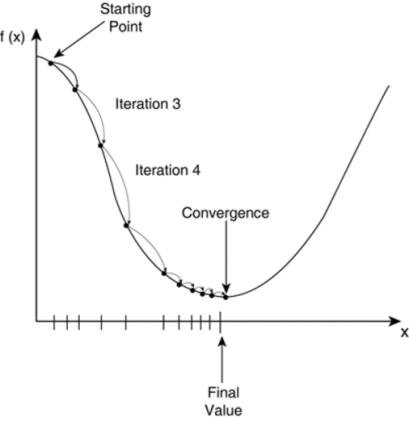
\includegraphics[width=\textwidth]{Sources/03-01_2_dimensionale_grafik_gd.png}
        \caption{2-dimensionaler Gradientenabstieg}
        \label{subsec:2-dimensionaler Gradientenabstieg}
        %TO-DO Quellennachweise einfügen(Abbildungsverzeichnis)
    \end{minipage}\hfill
    \begin{minipage}{0.45\textwidth}
        \centering
        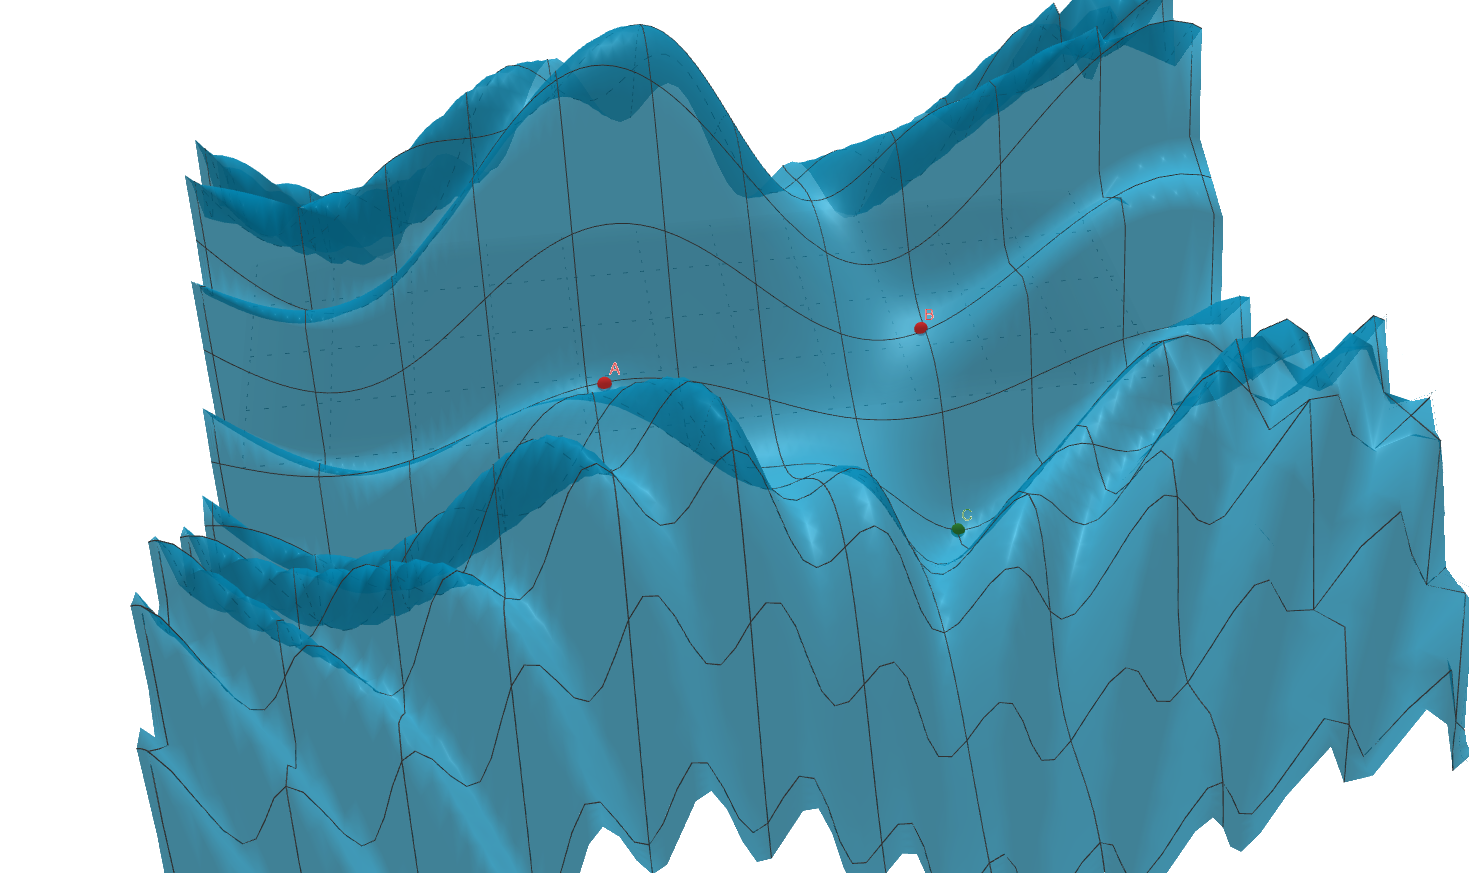
\includegraphics[width=\textwidth]{Sources/03-3.2.3_geogebra.png}
        \caption{3-dimensionaler Gradientenabstieg}
        \label{subsec:3-dimensionaler Gradientenabstieg}
        %TO-DO Quellennachweise einfügen(Abbildungsverzeichnis)
    \end{minipage}
\end{figure}
\newpage
 'Mathematisch ist der steilste Abstieg druch den sogenannten Gradienten(daher der Name Gradientenverfahren) repräsentiert bzw. genauer gesagt durch den negativen Gradienten, da der 
  Gradient selbst den stärksten Anstieg in der 'Hügellandschaft' makiert. Der Gradient gibt nicht nur die Richtung, sondern zugleich auch die Steigung des 'Hügels', sowie stellt folglich
  einen n-1-dimensionalen Vektor dar'\cite{GR10}.
\fi
\subsection{Gefährliche Fehlerquellen}\label{subsec:gradientenverfahren:fehlerquellen}
\subsubsection{Steckt man in einem lokalen Minimum fest?}\label{subsec:gradientenverfahren:fehlerquellen_lokalen_minimum}
  %\input{}
  Auf der Suche nach dem globalen Minimum kann der Algorithmus in einem lokalen Minimum enden und somit das Erreichen des globalen Minimums verhindert werden.
  Ein lokales Minimum tritt auf, wenn das Netzwerk an einem Punkt des Fehlergradienten auf eine niedrigere Fehlerfunktionsebene trifft, aber in der Nähe dieses Punktes ein anderer Punkt mit noch niedrigerem Fehler existiert (siehe Abb. 4).
  Da neurale Netze häufig große Anzahlen von Parametern haben, kann die Suche nach dem globalen Minimum eine schwierige Aufgabe sein \cite{HS97}.
  Oft wird in dieser Situation auch ein bergiges Gelände, in welchem eine Person, welche nur mit dem Strahl einer Taschenlampe ausgerüstet ist, zur Erklärung herangezogen \cite{TR17}.
  Diese Person kennt die Landschaft nicht, möchte aber den Fuß des Berges erreichen. Mit der Taschenlampe würde die Person den Boden ausleuchten, um der steilsten Neigung nach unten zu folgen.
  Sollte der Abstieg nicht weiter möglich sein, kann es sein, dass die einen Tiefpunkt erreicht hat, dieser aber nicht der tiefste Punkt der gesamten Landschaft ist.
  \\
  \begin{figure}[ht]
    \centering
    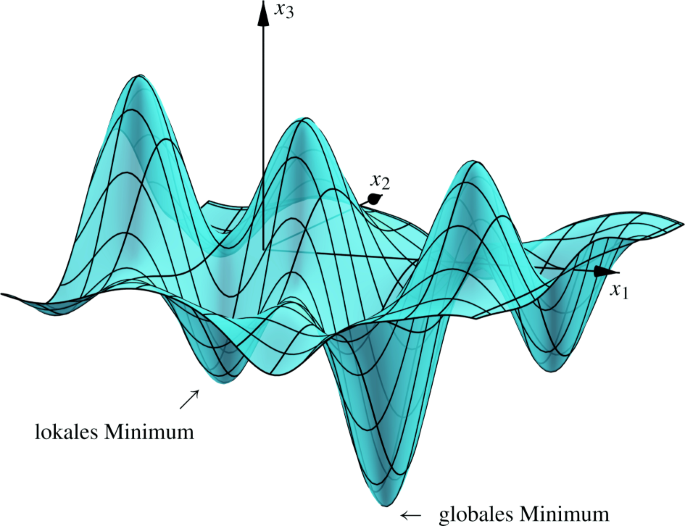
\includegraphics[width=0.5\textwidth]{Sources/03-3.3.2_3-dimensionaler_abstieg.png}
    \caption{Lokales und globales Minimum}
    \label{subsec:lokale-globale-minima}
\end{figure}

\subsubsection{Befindet man sich wirklich im globalen Minimum?}\label{subsec:gradientenverfahren:fehlerquellen_globalen_minimum}
  %\input{}
  Das Gradientenabstiegsverfahren finden in der Regel nur lokale Minima, abhängig vom gewählten Startpunkt \cite{HS97}.
  Durch die fehlende Kenntnis der gesamten (komplexen) Funktion ist es nicht sichergestellt, dass das Verfahren das globale Minimum (bzw. das tiefte Tal im Beispiel \ref*{subsec:gradientenverfahren:fehlerquellen_lokalen_minimum}) findet.

\subsubsection{Wie löst man dieses Problem?}\label{subsec:gradientenverfahren:fehlerquellen_problem_loesen}
Es stehen eine Liste an Änderungen am Gradientabstiegsverfahren zur Verfügung.
\begin{itemize}
  \item Initialisierung der Gewichte verändern:\\
  Man kann versuchen, die Initialisierung der Gewichte zu verändern, um den Lernerfolg zu verbessern. Dabei ist zu beachten, dass sowohl die Werte der Initialisierung für das Auffinden eines Minimums von Bedeutung ist, 
  als auch der Startpunkt $x^0\epsilon\mathbb{R}^n$ (\ref*{subsec:gradientenverfahren:wie_funktioniert}) des Gradientabstiegsverfahren, da dieser einen zentralen Einfluss darauf hat, welche Werte die Gewichte im Verlauf des Verfahrens annehmen. \\

  Zu beachten ist auch, dass die Initialisierung aller Gewichte auf denselben Zahlenwert dazu führt, dass die Gewichte in der Traininngsphase gleich verändert werden. Um diesem Problem entgegenzuwirken, wird die Initialisierung
  der Gewichte mit kleinen, um 0 herum streuenden Zufallsgewichten vorgenommen(symmetry breaking). \\
  Häufig kommt das sogenannte 'Multi-Start-Verfahren' zum Einsatz, bei dem die Berechnungen mit verschiedenen Startpunkten wiederholt werden. 
\end{itemize}
\begin{itemize}
  \item Lernparameter verändern:\\
  Neben Neu-Initialisierung der Gewichte kann der Lernparameter $\eta$ (\ref*{subsec:gradientenverfahren:wie_funktioniert}) verändert werden. Das Erhöhen des Lernparameters hat größere Sprünge zum Minimum zur Folge. Vorteil dabei ist, dass flache Plateaus schneller durchlaufen
  werden. Beim Minimieren des Lernparameters ergibt sich der Vorteil, dass das globale Minimum nicht mehr so leicht übersprungen werden kann. Dabei wäre jedoch ein Nachteil, dass das Gradientenverfahren eine deutlich längere Laufzeit bekommt.\\
  Eine oft angewandte Kombination ist daher, eine stufenweise Veränderung der Lernrate im Verlauf des Gradientenabstieges \cite[Seite 46]{GR10}.
\end{itemize}
\begin{itemize}
  \item Impuls-Term hinzufügen:\\
  Der Impuls-Term multipliziert zum aktuellen Gradienten den vorangegangenen Gradienten. Dadurch wird zusätzlich zur Berechnung ein Anteil $\alpha$ des vorherigen Gradient berücksichtigt.
  Dadurch kann das Verfahren schneller gegen das Minimum konvergieren und hilft, die Wahrscheinlichkeit von Schritten in die falsche Richtung zu reduzieren.

  Mit der Funktion aus \ref*{subsec:gradientenverfahren:wie_funktioniert} wäre die angewandte Änderung des Verfahrens dann:
  \begin{align*}
    \begin{bmatrix}
          x_{1}\\
          x_{2}\\
          \vdots \\
          x_{n}
         \end{bmatrix}_{Neu} = \alpha * \begin{bmatrix}
          x_{1}\\
          x_{2}\\
          \vdots \\
          x_{n}
         \end{bmatrix}_{Alt} - \eta \nabla f(x_{0})
  \end{align*}
  \noindent

  Folgende Vortile sind mit dem Impuls-Term verknüpft:
  \begin{itemize}
  \item Lokale Minima werden eher übersprungen
  \item Flache Plateaus werden aufgrund der Beschleunigung schneller durchlaufen.
  \end{itemize}
  Jedoch birgt der Einsatz davon auch die erhöhte Gefahr des Überspringen des globalen Minimums \cite{HS97}.
\end{itemize}
\noindent
Trotz der zahlreichen Lösungsmöglichkeiten, ist keine der Lösungen bei sämtlichen Problemen von Vorteil. 
Stattdessen ist oft simples ausprobieren notwendig, um die geeigneten Ansätze und Parameter auszuwählen. 
Ebenso können sich geeignete Methoden von Modell zu Modell unterscheiden \cite[Seite 48]{GR10}.

  
\thispagestyle{empty}
\section{Backpropagation}\label{sec:backpropagation}   

\vspace{1cm}
\begin{tcolorbox}[title={Inhalte der \textit{Backpropagation}}]
  \begin{quotation}\noindent
    Es wird ein Algorithmus gesucht, der die Wege ermittelt, welche einen stärkeren Einfluss auf den Output haben. Ebenso sollen diese Verbindungen dann gestärkt oder abgeschwächt werden.
    Dieses Kapitel erläutert, wie durch die Backpropagation ein neuronales Netz angepasst werden kann, um einen gewünschten Output zu erzielen. 
  \end{quotation}
  \begin{itemize}
    \item Was ist eine geeignete Verlustfunktion?
    \item Wie lernen Neuronale Netze?
    \item Grundidee Backpropagation
    \item Wie funktioniert der Backpropagation-Algorithmus
  \end{itemize}
\end{tcolorbox}

\subsection{Was ist eine geeignete Verlustfunktion?}\label{subsec:backpropagation:verlustfunktion}
Die Verlustfunktion wird genutzt um den Fehler eines neuronalen Netzes zu berechnen. Dieser Fehler gibt an, 
wie sehr die wirklichen Ausgabewerte des neuronalen Netzes nach Eingabe eines Trainingsdatensatzes von den gewollten Ausgabewerten abweichen. 
\bigbreak\noindent
Eine weitverbreitete Verlustfunktion ist der sogenannte Mean Squared Error (MSE), bei dem der Durchschnitt der quadrierten Fehler berechnet wird.
Bei Anwendung auf neuronale Netze lässt sich diese Funktion wie folgt ausdrücken:

\begin{eqnarray}  
  C(w,b) = \frac{1}{2n} \sum_x \| y(x) - a\|^2.
\end{eqnarray}

\noindent
In dieser Gleichung steht $w$ für die Gesamtheit aller Gewichte im neuronalen Netz, während $b$ alle Biases repräsentiert.
$n$ bezeichnet die Anzahl der Trainingsdatensätze und $y(x)$ ist der Vektor der Soll-Werte nach einem einzigen Trainingsbeispiel.
Schließlich ist $a$ der Vektor der tatsächlichen Ausgabewerte. 
\bigbreak\noindent
Wichtige Eigenschaften der MSE Verlustfunktion sind zum einen, dass sie niemals negativ wird, da jeder Term der Funktion positiv ist.
Außerdem sieht man recht einfach, dass $C(w, b) \approx 0$ gilt, wenn die die Soll-Werte ungefähr gleich den tatsächlichen Ausgabewerten sind.
\bigbreak\noindent
Es wird der durchschnittliche Fehler über \textbf{alle} Trainingsbeispiele berechnet. 
Es gibt Methoden, bei denen der Fehler nur für ausgewählte Teilgruppen (sog. Batches) von Trainingsbeispielen berechnet wird (Batch-Methode). 
Diese Vorgehensweise kann die Laufzeit des Backpropagation-Algorithmus verbessern, wird in diesem Text jedoch nicht weiter vertieft.
% TODO: Quelle angeben: http://neuralnetworksanddeeplearning.com/chap1.html#learning_with_gradient_descent

\subsection{Wie lernen Neuronale Netze?}\label{subsec:backpropagation:lernen_nn}
Da wir nun eine Verlustfunktion kennen, welche den Fehler eines neuronalen Netzes bestimmt, kann man eben jene
Verlustfunktion nutzen um das neuronale Netz lernen zu lassen. Der Ausgabewert der Verlustfunktion hängt sowohl von allen Weights $w$ 
als auch von allen Biases $b$ des neuronalen Netzes ab. Nun sucht man die konkreten Werte für die Weights und Biases, damit die 
Verlustfunktion so klein wie möglich wird. Dies tut man mit dem bereits oben beschriebenen Gradientenverfahren. Man braucht also den 
negativen Gradientenvektor der Verlustfunktion.
\cite{MN19}

\subsection{Grundidee Backpropagation}\label{subsec:backpropagation:grundiee}
Backpropagation stellt einen effizienten Algorithmus zur Berechnung dieses komplexen Gradientenvektors dar, den wir benötigen, um den Fehler in einem neuronalen Netzwerk zu minimieren.
Der Fehler an der Ausgabeschicht muss durch das gesamte Netz propagiert werden, um die Gewichte und Biaswerte entsprechend anzupassen.
Für jedes Gewicht und jeden Biaswert möchten wir bestimmen, wie stark der Fehler von diesem abhängt. 
Hierbei werden die partiellen Ableitungen verwendet, die die Sensitivität einer Funktion in Bezug auf eine Änderung einer bestimmten Variable messen.
Konkret suchen wir nach den Werten von $\frac{\partial C}{\partial w_{jk}^{l}}$ und $\frac{\partial C}{\partial b_{j}^{l}}$, die partiellen Ableitungen der Kostenfunktion (C) nach den Gewichten ($w_{jk}^{l}$) und Biaswerten ($b_{j}^{l}$).
\cite{MN19}

\subsection{Wie funktioniert der Backpropagation-Algorithmus}\label{subsec:backpropagation:fehlerrueckfuehrung}
Für die Erklärung des Backpropagation-Algorithmus nehmen wir folgendes neuronales Netz an:
\begin{figure}[H]
  \centering
  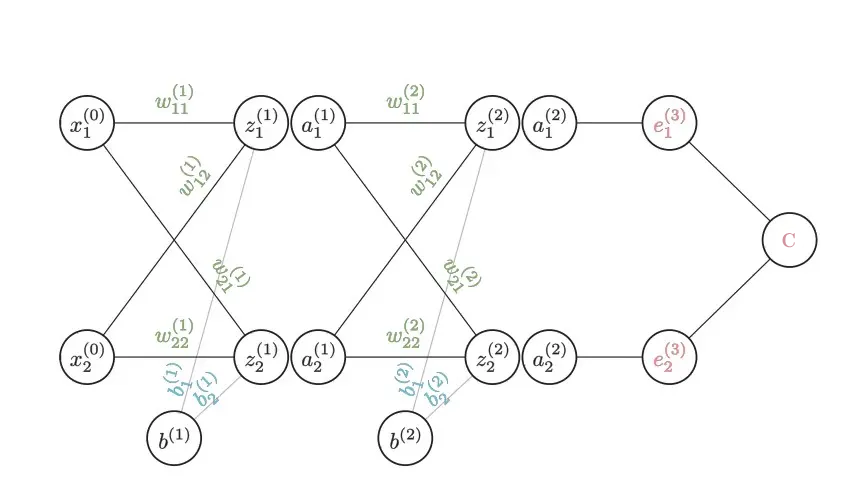
\includegraphics[width=0.5\textwidth]{Sources/04-05_backprop_nn_example.png}
  \caption{Quelle: https://towardsdatascience.com/understanding-backpropagation-abcc509ca9d0}
\end{figure}
\noindent
Der gesamte Fehler $C$ wurde in der Abbildung auf die zwei Output-Neuronen über $e_1^{(3)}$ und $e_2^{(3)}$ aufgeteilt.
Außerdem wurde jedes Hidden-Neuron in seine gewichtete Summe $z$ und seine Aktivierungsfunktion $a$ aufgeteilt.
Zuerst muss man sich überlegen, wie man die Weights / Biases, welche in die Output-Schicht einfließen anpasst.
Wenn man nun beispielsweise ausrechnen möchte welchen Einfluss das Gewicht $w_{11}^{(2)}$ auf den Fehler C hat, dann muss man 
$\frac{\partial C}{\partial w_{11}^{(2)}}$ berechnen. Hierfür macht es Sinn, dass man sich anschaut wie das Weight $w_{11}^{(2)}$ in den Fehler C einfließt.
Das Gewicht $w_{11}^{(2)}$ geht nur in den Teilfehler $e_1$ ein, daher muss man auch nur diesen betrachten.
\begin{flalign*}  
  e_{1}^{(3)} &= (y(x) - a_1^{(2)})^2\\
  a_{1}^{(2)} &= \sigma(z_{1}^{(2)})\\
  z_{1}^{(2)} &= w_{11}^{(2)} * a_{1}^{(1)} + w_{12}^{(2)} * a_{2}^{(1)} + b_1^{(2)}\\
  \Rightarrow e_{1}^{(3)} &= (y(x) - \sigma(w_{11}^{(2)} * a_{1}^{(1)} + w_{12}^{(2)} * a_{2}^{(1)} + b_1^{(2)}))^2
\end{flalign*}
\noindent
Möchte man nun die oben genannte partielle Ableitung ausrechnen, dann macht man sich die Kettenregeln zu Nutze und es gilt: 
\begin{align*}  
  \frac{\partial C}{\partial w_{11}^{(2)}} = \frac{\partial e_1^{(3)}}{\partial a_1^{(2)}}\frac{\partial a_1^{(2)}}{\partial z_{1}^{(2)}}\frac{\partial z_{1}^{(2)}}{\partial w_{11}^{(2)}}
\end{align*}
\noindent
Diesen Schritt würde man für jedes Weight ausführen, welches in ein Output-Neuron einfließt.
Anstatt jede partielle Ableitung einzeln aufzuschreiben macht man sich das Hadamard-Produkt zu Nutze um effizient alle partiellen
Ableitungen dieser Weights zu berechnen:
\begin{align*}
  \renewcommand{\arraystretch}{1.5}
  \begin{bmatrix}
    \frac{\partial C}{\partial w_{11}^{(2)}} & \frac{\partial C}{\partial w_{12}^{(2)}} \\
    \frac{\partial C}{\partial w_{21}^{(2)}} & \frac{\partial C}{\partial w_{22}^{(2)}} \\
  \end{bmatrix} = 
  \begin{bmatrix}
    \frac{\partial e_1^{(3)}}{\partial a_1^{(2)}} \\
    \frac{\partial e_2^{(3)}}{\partial a_2^{(2)}}
  \end{bmatrix} \odot 
  \begin{bmatrix}
    \frac{\partial a_1^{(2)}}{\partial z_1^{(2)}} \\
    \frac{\partial a_2^{(2)}}{\partial z_2^{(2)}}
  \end{bmatrix} \odot
  \begin{bmatrix}
    \frac{\partial z_1^{(2)}}{\partial w_{11}^{(2)}} & \frac{\partial z_1^{(2)}}{\partial w_{12}^{(2)}} \\
    \frac{\partial z_2^{(2)}}{\partial w_{21}^{(2)}} & \frac{\partial z_2^{(2)}}{\partial w_{22}^{(2)}} \\
  \end{bmatrix}
  \renewcommand{\arraystretch}{1}
\end{align*}
\noindent
Die zwei linken Vektoren des Hadamard-Produkts werden im folgenden noch zu einem $\delta$ Term zusammengefasst, da diese in späteren 
Berechnungen öfters auftreten.
\begin{align*}
  \delta^{(L)} = \frac{\partial C}{\partial A^{(2)}} \odot \frac{\partial A^{(2)}}{\partial Z^{(2)}}\\
  \\
  \Rightarrow \frac{\partial C}{\partial W^{(2)}} = \delta^{(L)} \odot \frac{\partial Z^{(2)}}{\partial W^{(2)}}
\end{align*}
\noindent
Jetzt muss man sich noch anschauen wie man die Abhängigkeit des Fehlers eines tiefer liegenden Weights / Biases 
berechnet, z.B. $\frac{\partial C}{\partial w_{11}^{(1)}}$. Die Grundidee bleibt die selbe, jedoch können nun mehrere Pfade vom gesamten Fehler 
zu diesem Weight führen. In diesem Fall addieren wir die Kettenregel-Terme beider Pfade zusammen, bis sie sich an einem Neuron treffen.
\begin{align*}  
  \frac{\partial C}{\partial w_{11}^{(1)}} = (\frac{\partial e_1^{(3)}}{\partial a_1^{(2)}}\frac{\partial a_1^{(2)}}{\partial z_1^{(2)}}\frac{\partial z_1^{(2)}}{\partial a_1^{(1)}} + \frac{\partial e_2^{(3)}}{\partial a_2^{(2)}}\frac{\partial a_2^{(2)}}{\partial z_2^{(2)}}\frac{\partial z_2^{(2)}}{\partial a_1^{(1)}})
  \frac{\partial a_1^{(1)}}{\partial z_1^{(1)}}\frac{\partial a_1^{(1)}}{\partial w_{11}^{(1)}}
\end{align*}
In dieser Gleichung sieht man nun auch die sich wiederholenden $\delta^{L}$ Terme.
\begin{align*}  
  \frac{\partial C}{\partial w_{11}^{(1)}} = (\delta_1^{L}\frac{\partial z_1^{(2)}}{\partial a_1^{(1)}} + \delta_2^{L}\frac{\partial z_2^{(2)}}{\partial a_1^{(1)}})
  \frac{\partial a_1^{(1)}}{\partial z_1^{(1)}}\frac{\partial a_1^{(1)}}{\partial w_{11}^{(1)}}
\end{align*}
\noindent
Auch diese Berechnung führen wir für jedes "tiefere" Weight (in dem Fall von der 1. zur 2. Schicht) aus. Durch Matrizen lässt sich diese Berechnung wiefolgt ausdrücken: 
\begin{align*}
  \renewcommand{\arraystretch}{1.5}
  \begin{bmatrix}
    \frac{\partial C}{\partial w_{11}^{(1)}} & \frac{\partial C}{\partial w_{12}^{(1)}} \\
    \frac{\partial C}{\partial w_{21}^{(1)}} & \frac{\partial C}{\partial w_{22}^{(1)}}
  \end{bmatrix} = \begin{bmatrix}
   \delta_1^L \\
   \delta_2^L
  \end{bmatrix}^T \cdot  
  \begin{bmatrix}
    \frac{\partial z_1^{(2)}}{\partial a_1^{(1)}} & \frac{\partial z_1^{(2)}}{\partial a_2^{(1)}}\\
    \frac{\partial z_2^{(2)}}{\partial a_1^{(1)}} & \frac{\partial z_2^{(2)}}{\partial a_2^{(1)}}
  \end{bmatrix} \odot 
  \begin{bmatrix}
    \frac{\partial a_1^{(1)}}{\partial z_1^{(1)}} \\
    \frac{\partial a_2^{(1)}}{\partial z_2^{(1)}}
  \end{bmatrix} \odot
  \begin{bmatrix}
   \frac{\partial z_1^{(1)}}{\partial w_{11}^{(1)}} && \frac{\partial z_1^{(1)}}{\partial w_{12}^{(1)}}\\
   \frac{\partial z_2^{(1)}}{\partial w_{21}^{(1)}} && \frac{\partial z_2^{(1)}}{\partial w_{22}^{(1)}}
  \end{bmatrix}
  \renewcommand{\arraystretch}{1.0}
\end{align*}
\begin{align*}
  \Rightarrow \frac{\partial C}{\partial W^{(1)}} = (\delta^L)^T \cdot \frac{\partial Z^{(2)}}{\partial A^{(1)}} \odot
  \frac{\partial A^{(1)}}{\partial Z^{(1)}} \odot \frac{\partial Z^{(1)}}{\partial W^{(1)}}
\end{align*}
\noindent
Die Berechnungen für die Bias-Werte sehen sehr ähnlich aus, daher werden diese hier nicht weiter ausgeführt.
Somit kommt man auf die allgemeinen Formeln für die Backpropagation: 
\begin{flalign*}
  \frac{\partial C}{\partial W^{(l)}} &= (\delta^{(l+1)})^T \cdot W^{(l+1)} \odot \frac{\partial A^{(l)}}{\partial Z^{(l)}} \odot X^{(l - 1)}\\
  \delta^{(L)} &= \frac{\partial C}{\partial A^{(L)}} \odot \frac{\partial A^{(L)}}{\partial Z^{(L)}}\\
  \frac{\partial C}{\partial B^{l}} &= \delta^l
\end{flalign*}
\cite{MN19}

  \newpage
\thispagestyle{empty}
\section{Trainings- und Testdaten}\label{sec:training_testdaten}   
\begin{tcolorbox}[title={Inhalte von \textit{Trainings- und Testdaten}}]
  \begin{quotation}\noindent
    Im letzten Kapitel wird auf die Datensätze eingegangen, welche genutzt werden, um ein Modell zu trainieren.
  \end{quotation}
  \begin{itemize}
    \item Trainieren und Testen von Neuralen Netzen?


  \end{itemize}
\end{tcolorbox}

\section{Trainieren und Testen von Neuralen Netzen}\label{sec:trainingsdaten}   
Zum Trainieren eines Modells wird ein Datensatz benötigt. Dieser Datensatz wird in der Regel in mindestens drei verschiedene Datensätze unterteilt: Training-, Validierung- und Testdaten.
Hier kann die Frage aufkommen, warum diese Unterteilung gemacht wird und nicht der vollständige Datensatz zum Lernen verwendet wird. 
Diese Frage sollte bei der Erklärung der Verwendungszwecke der jeweiligen Daten beantwortet werden

\subsection{Trainingsdaten}
Ein Trainingsdatensatz ist ein Datensatz mit Beispielen. Konkret bedeutet das, dass hier eine Zuordnung zwischen Input -> Output bereits gegeben ist. 
Diese Daten werden genutzt, um die Gewichte (siehe \ref*{subsec:neuronen:verknuepfung_neuronen:Weights}) des neuronalen Netzes anzupassen.
In der Literatur wird dieser Teil mit 70 bis 80 Prozent von der gesamten Datenmenge bemessen.

\subsection{Validierungsdate}
Der Validierungsdatensatz dient dazu, die Leistung des Modells während des Trainings zu bewerten und die Parameter (z.B. Lernrate oder Gewichte) zu optimieren. 
Dadurch wird das Modell verbessert.
In der Literatur wird dieser Teil mit 10 Prozent von der gesamten Datenmenge bemessen.

\subsection{Testdaten}
Mithilfe des Testdatensatzes wird die Qualität des neuronalen Netzes nach dem Training überprüft. Wichtig ist dafür, dass dieser Datensatz zuvor nicht zum Lernen verwendet wurde, 
damit diese das Ergebnis nicht verfälschen.
So kann festgestellt werden, wie das Modell auf Daten reagiert, welche nicht zuvor trainiert wurden.
In der Literatur wird dieser Teil mit 10 bis 15 Prozent von der gesamten Datenmenge bemessen.


Insgesamt sollte nun klar sein, warum die Datensätze vollständig getrennt verwendet werden sollten. 
Wichtig anzumerken ist noch, dass die Verteilung der Datensätze variiert und so gewählt werden sollte, dass das Modell ausreichend gut trainiert, validiert und robust getestet wird.

\subsection{Problem: Overfitting}
Overfitting tritt auf, wenn das neuronale Netz zu stark an die Trainingsdaten angepasst ist und nicht gut auf neue, unbekannte Daten reagiert. 
Bei einer nur geringen Anzahl an Trainingsdaten werden nicht genug Anpassungen durchgeführt, sodass ein Lernen nach Mustern möglich wird. Die Folge davon ist, dass die Trainingsdaten auswendig gelernt werden.
Dadurch hat das neuronale Netz eine sehr hohe Genauigkeit bei den Trainingsdaten, jedoch eine sehr geringe bei dem Validierungsdatensatz. 
    

  % Quellenverzeichnis
  \newpage
  \thispagestyle{empty}
  \section{Quellenverzeichnis}
    \subsection{Literatur}
    \renewcommand{\refname}{} % Literaturverzeichnis ohne Bezeichnung
    % Variante 1: einfaches, manuelles 
    % Literaturverzeichnis
    \begin{thebibliography}{SW11} % 2. {...} => Hier die größte /breiteste Nummer (z.B. 99) oder Kurzbeleg angeben.
      \bibitem[SW11]{SW11} Stickel-Wolf, Christine; Wolf, Joachim (2011): Wissenschaftliches Lernen und Lerntechniken. Erfolgreich studieren–-gewusst wie!. Wiesbaden: Gabler. 
      \bibitem[CA18]{CA18} Aggarwal, Charu C. (2018): Neural Networks and Deep Learning: A Textbook. Springer.
      \bibitem[TR17]{TR17} Rashid, Tariq (2017): Neuronale Netze selbst programmieren. In O`Reilly eBooks. NY, USA
      \bibitem[GBCL18]{GBCL18} Goodfellow, I., Bengio, Y., Courville, A., \& Lenz, G. (2018): "Deep Learning: das umfassende Handbuch : Grundlagen, aktuelle Verfahren und Algorithmen, neue Forschungsansätze." 1. Auflage. Frechen: mitp. ISBN 978-3-95845-701-0.
    \end{thebibliography} 
        
    \subsection{Internetquellen}
    \begin{thebibliography}{HR08} % 2. {...} => Hier die größte/breiteste Nummer (z.B. 99) oder Kurzbeleg angeben.
      \bibitem[BBoJ]{BBoJ} Bertelsmeier, Birgit (o. J.): Tipps zum Schrei\-b\-en ei\-n\-er Ab\-sch\-luss\-ar\-beit. Fach\-hoch\-schu\-le Köln-Campus Gummersbach, Institut für Informatik. \url{http://lwibs01.gm.fh-koeln.de/blogs/bertelsmeier/files/2008/05/abschlussarbeitsbetreuung.pdf} (29.10.2013).
      \bibitem[HR08]{HR08} Halfmann, Marion; Rühmann, Hans (2008): Merkblatt zur Anfertigung von Projekt-, Bachelor-, Master- und Diplomarbeiten der Fakultät 10. Fachhochschule Köln-Campus Gummersbach.\url{http://www.f10.fh-koeln.de/imperia/md/content/pdfs/studium/tipps/anleitungda270108.pdf} (29.10.2013).
      \bibitem[JH20]{JH20} Harrer, J. (2020): Künstliche Neuronale Netze.\url{https://pxldeveloper.eu/assets/docs/KuenstlicheNeuronaleNetzeJulianHarrer.pdf} (20.04.2023)
      \bibitem[GR10]{GR10} Günter Daniel Rey und Karl F Wender(2010): Neuronale Netze, eine Einführung in die Grundlagen, Anwendung und Datenauswertung
      \bibitem[HS97]{HS97} Hochreiter, S. and Schmidhuber, J. (1997): Flat minima. Neural Computation, 9(1), 1-42.
      \bibitem[LH21]{LH21} Linus Henning: Gradienten Verfahren zur Optimierung Neuronaler Netze. Weierstraß-Institut für Angewandte Analysis und Stochastik. \url{https://www.wias-berlin.de/people/john/BETREUUNG/bachelor_henning.pdf} (12.10.2021)
    \end{thebibliography} 
  
  % INFO: Biblatex -Ausgabe des  
  % Literaturverzeichnisses (Beispiele):   
  % - \printbibliography => Ausgabe ALLER 
  %   Einträge
  % - \printbibliography[nottype=online]
  %   => Ausgabe der Einträge, bis auf die
  %      "Online"-Einträge
  % - \printbibliography[type=online]     
  %   => Ausgabe nur der "Online"-Einträge  
  % \printbibliography

  % Anhang
  %% Anhang
\newpage
\setcounter{section}{0} % Nummerierung der Gliederungsebene "section" auf 0 setzen
\renewcommand*\thesection{\Alph{section}} % Nummerierungsart für die Gliederungsebene "section" 
% auf Großbuchstaben setzen
\section{Anhang}\label{anhang}
\subsection{Unterabschnitt von Anhang}\label{subsec_UabsAnhang}
TEXT FOLGT...
  
  % % Erklärung über die selbständige Abfassung der Arbeit  
\newpage
\pagestyle{empty}
\section*{Erklärung über die selbständige\\Abfassung der Arbeit} % \section*{...}: das *-Symbol erlaubt, dass dieser
% Gliederungspunkt nicht ins Inhaltsverzeichnis aufgenommen wird
\addcontentsline{toc}{section}{Erklärung über die selbständige Abfassung der Arbeit}
Ich versichere, die von mir vorgelegte Arbeit selbständig verfasst zu haben.
Alle Stellen, die wörtlich oder sinngemäß aus veröffentlichten oder nicht veröffentlichten Arbeiten anderer entnommen sind,
habe ich als entnommen kenntlich gemacht.\\ 
Sämtliche Quellen und Hilfsmittel, die ich für die Arbeit benutzt habe, sind
angegeben. Die Arbeit hat mit gleichem Inhalt bzw. in wesentlichen Teilen noch keiner anderen Prüfungsbehörde vorgelegen.\\\\
\begin{tabular}{cp{7cm}}
    & \\ 
    & \\ \hline
    \small (Ort, Datum, Unterschrift) & \normalsize \\
    \end{tabular}
    
    %<MERKKASTEN> (für die eigene Verwendung bitte entfernen
    \vspace{1cm}
\begin{tcolorbox}[title={Hinweise zur obigen \textit{Erklärung}}]
\begin{itemize}
\item Bitte verwenden Sie nur die Erklärung, die Ihnen Ihr \textbf{Prüfungsservice} vorgibt. Ansonsten könnte es passieren, dass Ihre Abschlussarbeit nicht angenommen wird. Fragen Sie im Zweifelsfalle bei Ihrem Prüfungsservice nach.
\item Sie müssen \textbf{alle abzugebende Exemplare} Ihrer Abschlussarbeit unterzeichnen. Sonst wird die Abschlussarbeit nicht akzeptiert. 
\item Ein \textbf{Verstoß} gegen die unterzeichnete \textit{Erklärung} kann u.\,a. die Aberkennung Ihres akademischen Titels zur Folge haben.
\end{itemize}  
\end{tcolorbox}
%</MERKKASTEN>   
  
  % Unbeschriftetes Abschlussblatt (Leere Seite)
  %\newpage
  %\thispagestyle{empty}
  %\newpage
\thispagestyle{empty}
\section*{}
 
    
\end{document}